\section{Requirement Gathering and analysis}\label{sec:rga}
The collection and analysis of requirements is the first phase in the SDLC process. The methodologies employed in this stage included interviews, questionnaires, and observational data collection to obtain requirements. We have divided all of the needs into two categories: functional requirements and non-functional requirements. Functional requirements are those that are necessary for the application to operate.
\subsection{Requirement Gathering}\label{sub:reqgather}
\subsubsection{Functional Requirements:}\label{subsub:funreq}
To collect functional requirements, we met some teachers from our university and interviewed them. The following are some of their requirements:
\begin{itemize}
	\item Less time-consuming attendance system.
	\item Attendance statistics in detail  should be easy to calculate (From teachers and students ends).
	\item Attendance system must be transparent.
	\item Students' records should be printable.
	\item Less paperwork and one-click procedure.
\end{itemize}
Then we meet some administrative officers to meet their requirements and interviewed them. Their requirements include the following things:
\begin{itemize}
	\item Students must be able to enter transaction data into a user interface accepts transaction data.
	\item Students will be able to make fee payments online.
	\item Students should be able to receive feedback on the  online payment.
	\item If the fee payment transaction is successful, students can view, print, or save the payment receipt.
	\item Financial officers will be permitted to lead look on the data of individuals online payment information.
	\item The finance officer will be able to view statistics of all payments made through the system.
	\item Financial officers will be permitted to look at the data of individuals' online payment information.
	\item Finance officials will be able to see fee payments in an editable manner.
\end{itemize}
Secondly, we conducted a survey among all the students of the University of Chittagong to meet their requirements. According to the survey we have come out with some requirements such as:
\begin{itemize}
	\item Less time-consuming attendance and payment system
	\item Being free from working hours 
	\item Get rid of the tiresome process of queuing
	\item Expanding the ways of transaction
	\item Being independent of a specific bank branch
	\item Being able to make transactions from anywhere
\end{itemize}

\subsubsection{Non-Functional Requirements:}\label{subsub:nonfunreq}
According to the interviews of administrative officers and teachers and the survey conducted on students of the University of Chittagong as well as our observation we did find out some non-functional requirements which are as followings:
\begin{itemize}
	\item The system must be easy to operate.
	\item User interface should be simple and understandable for both experienced and inexperienced users.
	\item The system must be secured enough.
	\item Speed of the system should be as fast as possible.
	\item It should be cross-platform compatible.
	\item Reports should be provided in a variety of formats, such as tables and graphs, for simple management visualization.
	\item A standard graphical user interface that facilitates online data entry, modification, update, and deletion.
\end{itemize}
\subsection{Requirement Analysis}\label{sub: reqana}
Following the collection of requirements, the next stage is to examine them. We have accomplished this stage in accordance with Structured Analysis Methodologies, which focuses on the functional decomposition and data-flow analysis, among other things. Following the brainstorming session of our team, we came up with a context diagram that is easier to understand.\\
\begin{figure}[H]
    \centering
    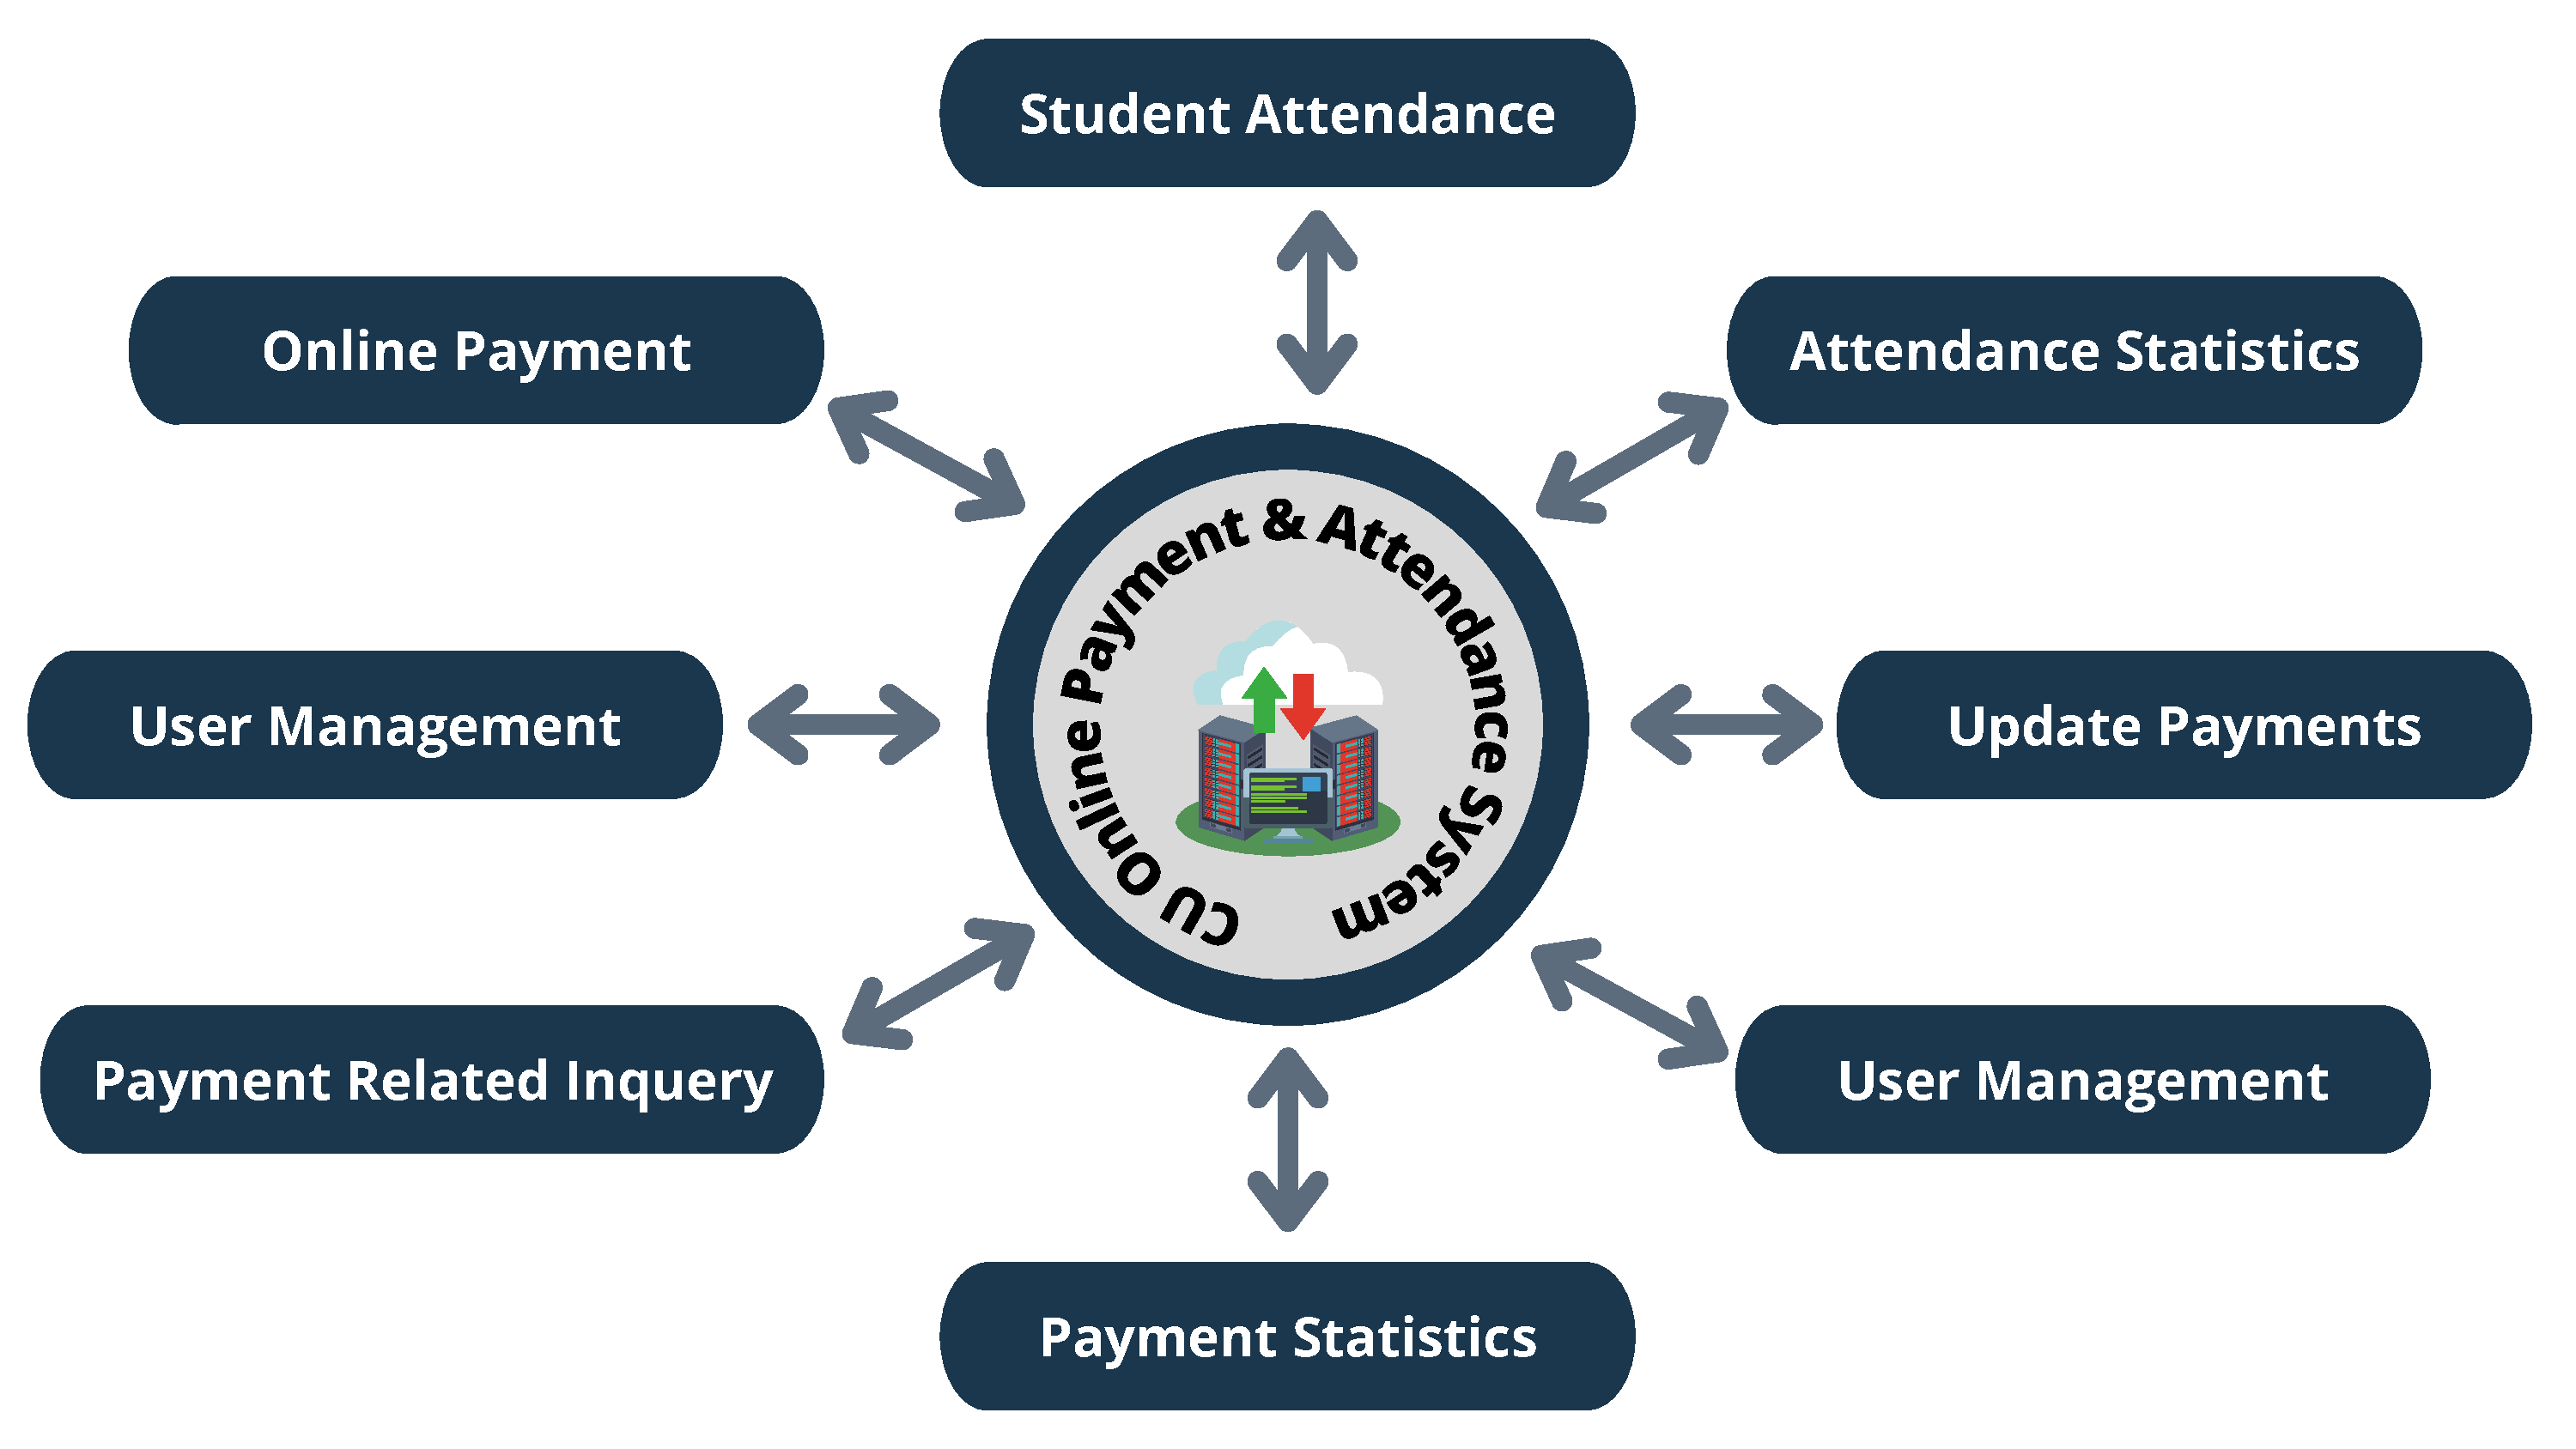
\includegraphics[width=1\textwidth]{images/context}
    \caption{Context Diagram of CU-OPAS}
    \label{fig:context}
\end{figure}
We brought it up in front of the appropriate authorities as well as our supervisor. Then it was slightly tweaked to make it more user-friendly. Finally, we completed a model of the system that meets all of the needs of administrative authorities, instructors, and students, and it is ready for implementation. A flowchart was then built in order to define the sequence of actions.\\
\begin{figure}[H]
    \centering
    \label{fig:flowchart}
    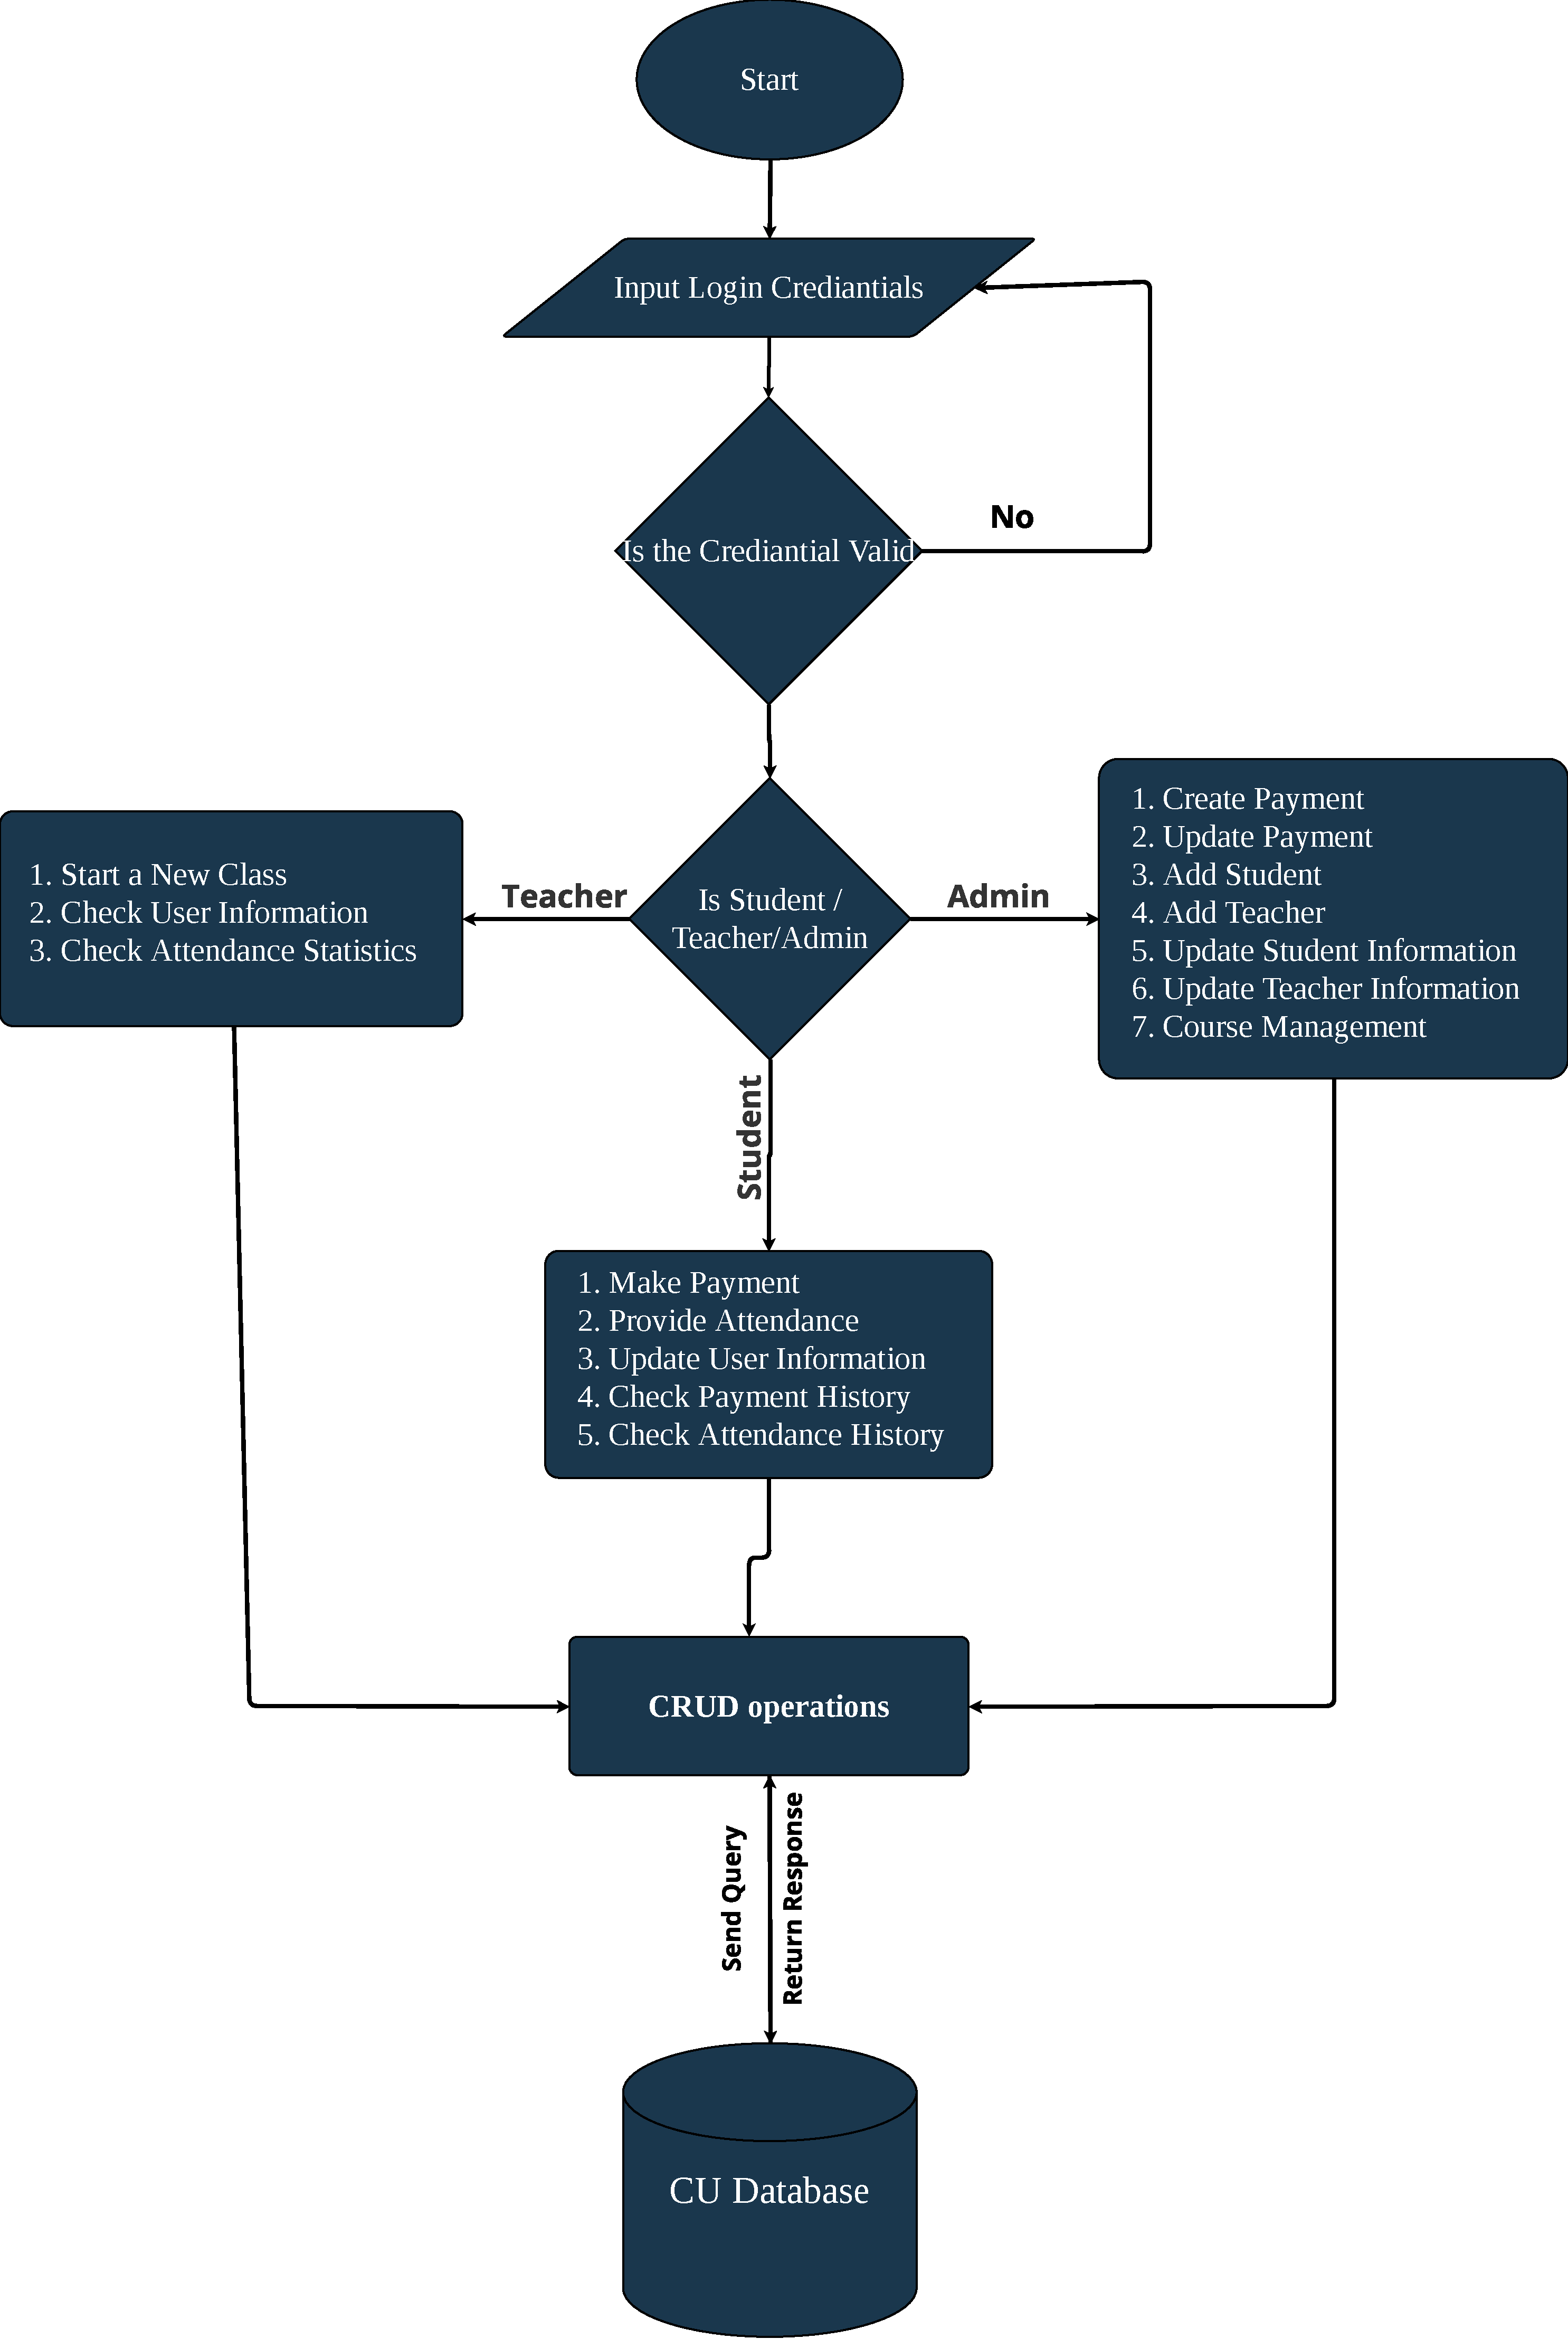
\includegraphics[height=15cm, width=1\textwidth]{images/flowchart}
    \caption{Flowchart of CU-OPAS}
\end{figure}
Finally, we have a completed entity relationship diagram that is ready for implementation.
\begin{figure}[H]
    \centering
    \label{fig:erd}
    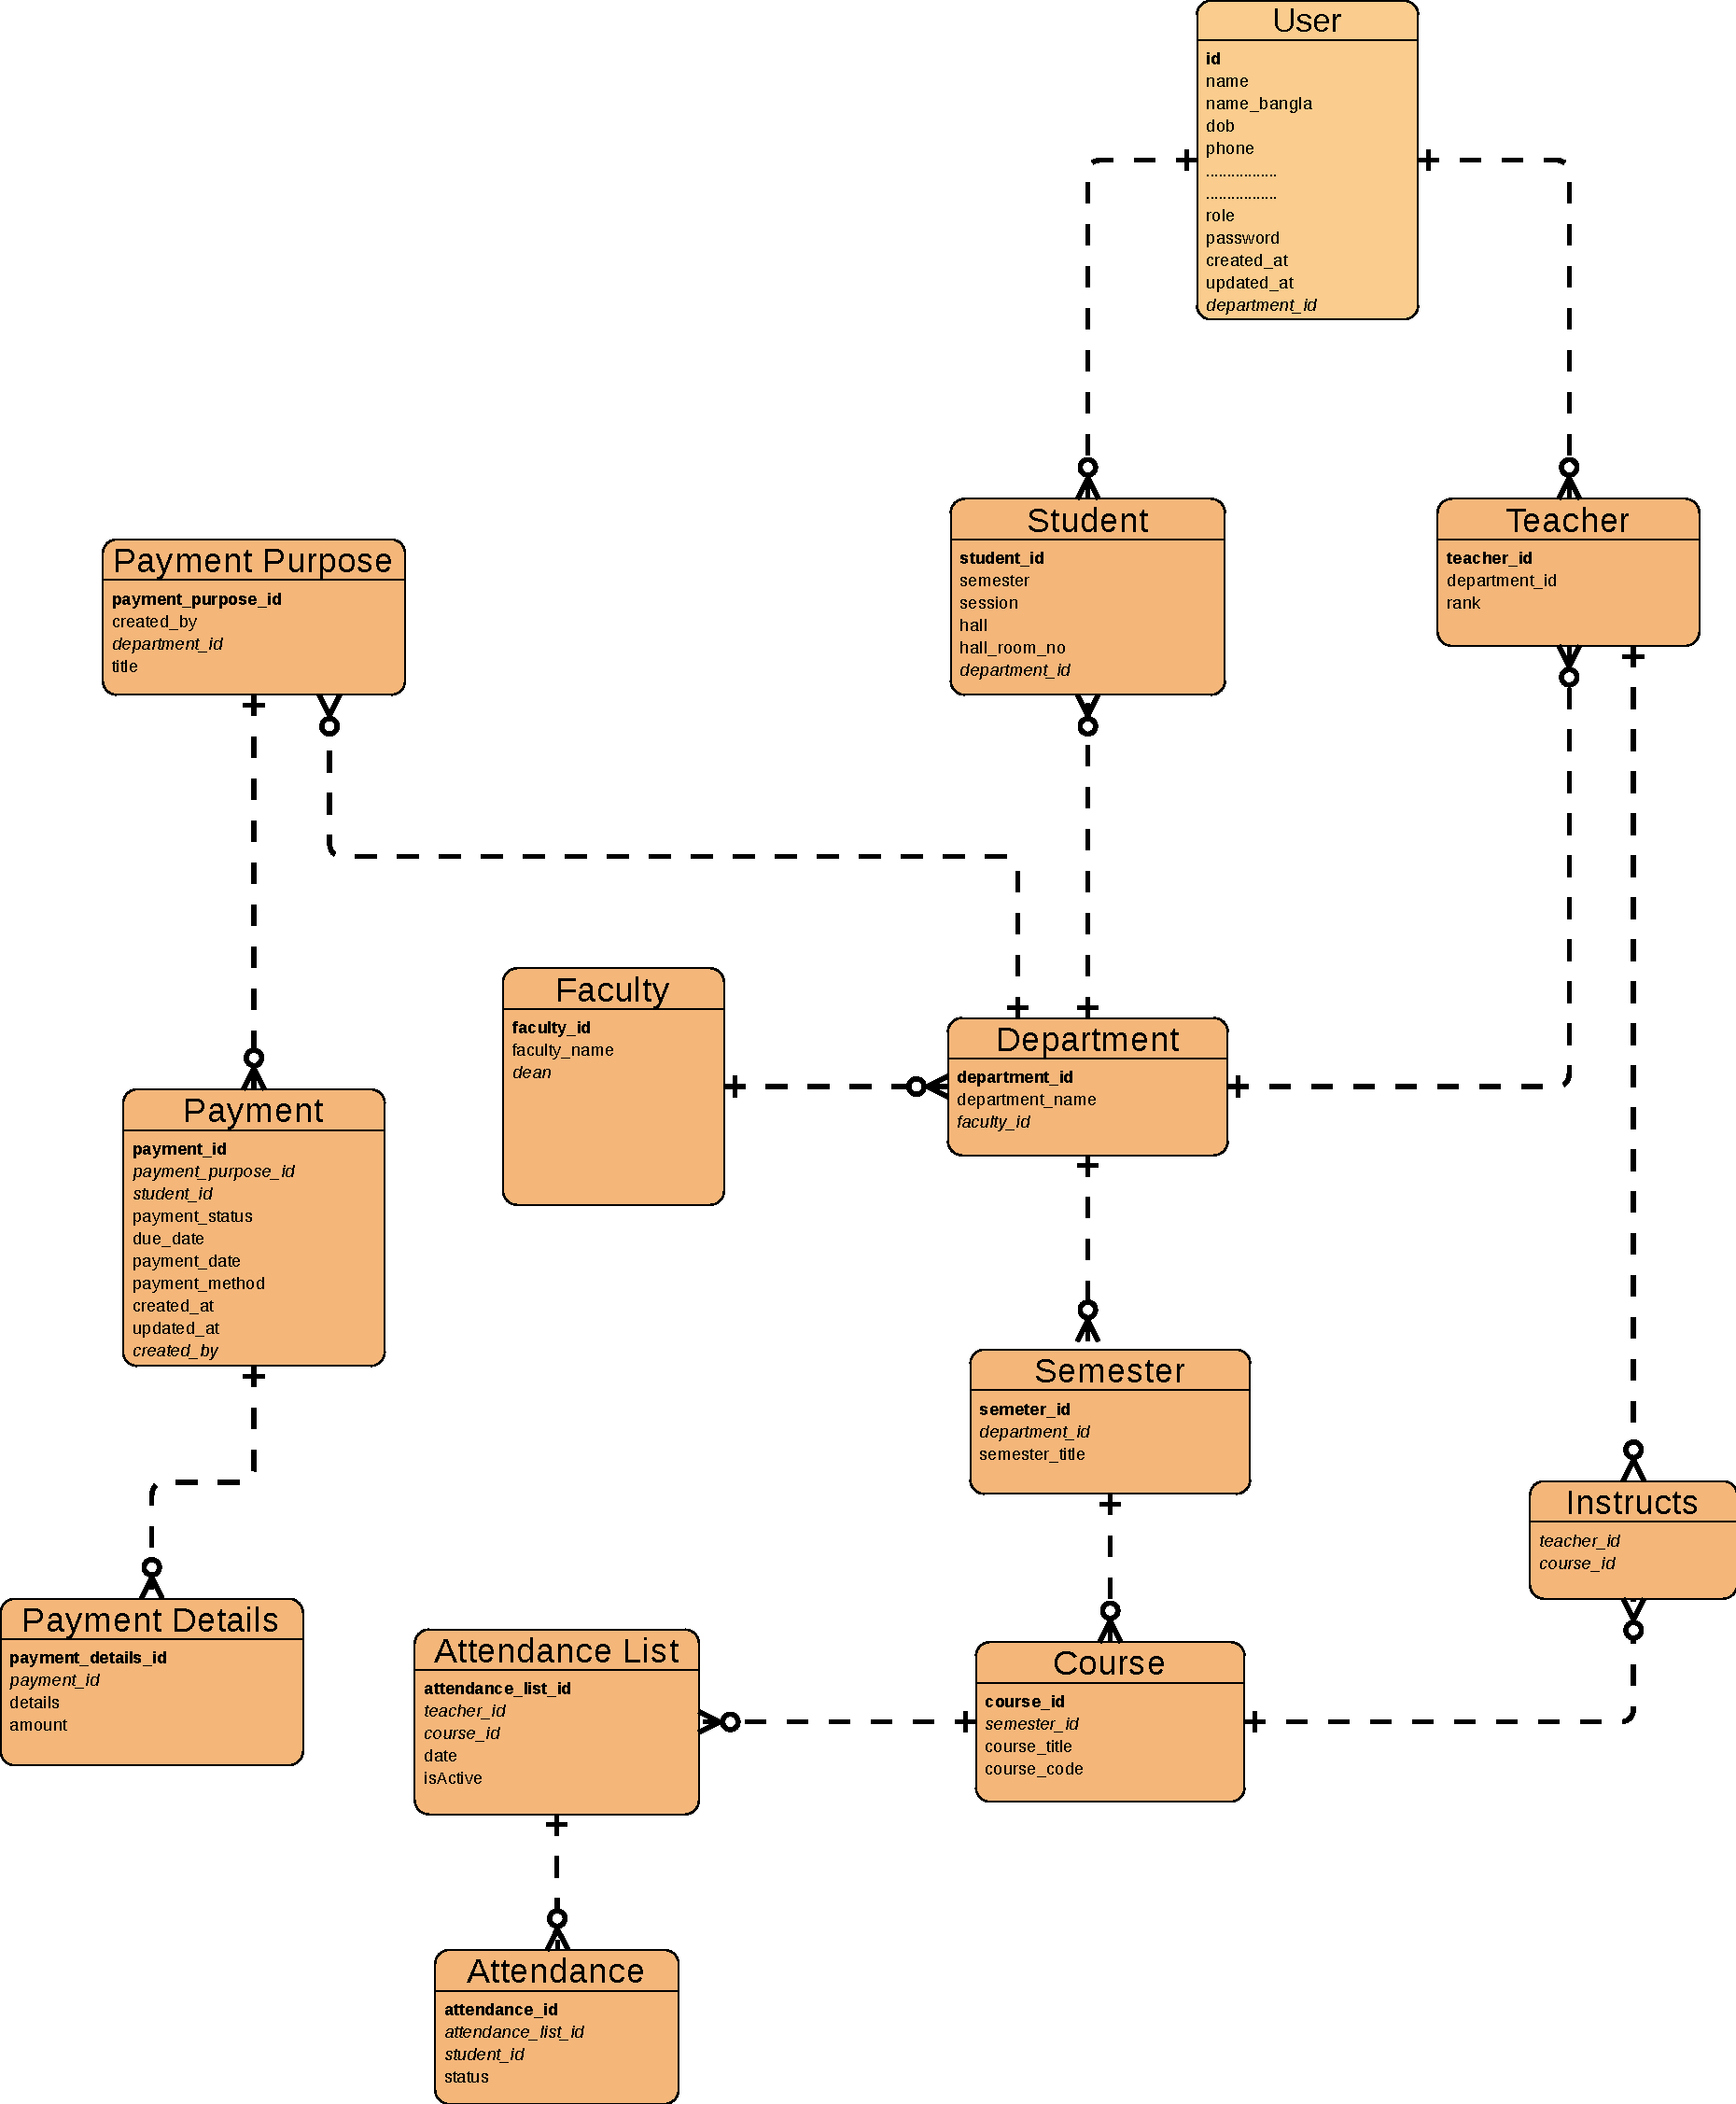
\includegraphics[width=1\textwidth]{images/erd}
    \caption{Entity Relationship Diagram of CU-OPAS}
\end{figure}
Stakeholders are the individuals that are involved in the project. There is apprehension regarding the project's result among them. Stakeholders may also include a group, a firm, customers, suppliers, and other parties. Every stakeholder has an effect on the project, either directly or indirectly. According to this classification, there are two sorts of stakeholders: primary and secondary. In this project, the key stakeholders are supervisors, team members, teachers, and administrative authorities, while the secondary stakeholders include students, the news media, and other teams.
\clearpage